%!TEX root = ../../Main.tex
\graphicspath{{Chapters/Vippefunktionalitet/}}
%-------------------------------------------------------------------------------

\chapter{Applikation::server}
Ligesom med clienten er koden taget fra øvelse 7 og tilpasset vores nye system. 

Serveren modtager et navn på en fil og sender den med det samme tilbage til clienten. 

\begin{lstlisting}[frame=single]  % Start your code-block

file_server::file_server ()
{
    Transport::Transport * myTransport = new Transport::Transport(BUFSIZE);
    char buffer[BUFSIZE] = {0};
    long fsize;


    CORRUPT_DATA = 2;
    CORRUPT_ACK = 2;

    /*Modtager filnavn*/
    myTransport->receive(buffer,BUFSIZE);
    std::cout << "Forspurgte fil: " << buffer << std::endl;
    string fileName_(buffer);

    /*Soeger efter filen*/
    struct stat sts;
    if ((stat (buffer, &sts)) == -1)
    {
        fprintf(stderr,"Fejl: Filen findes ikke. \n");
        fsize = 0;
    }
    else
    {
        fsize = sts.st_size;
        printf("Fil stoerrelse: %d \n", fsize);
    }

  
    sprintf(buffer,"%d",fsize);
    myTransport->send(buffer, sizeof(buffer));

    if(fsize == 0)
    {
        exit(0);
    }


    /*Sender fil*/
    sendFile(fileName_,fsize,myTransport);

}
\end{lstlisting}


\begin{figure}[H]
\centering
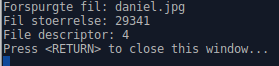
\includegraphics[width = 300 pt]{Img/server.PNG}
\caption{Server}
\label{fig:konceptbillede}
\end{figure}

\begin{figure}[H]
\centering
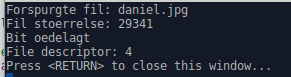
\includegraphics[width = 300 pt]{Img/korrupt_data.PNG}
\caption{Server korrupt data}
\label{fig:konceptbillede}
\end{figure}

\begin{figure}[H]
\centering
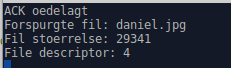
\includegraphics[width = 300 pt]{Img/ack_broke.PNG}
\caption{Server korrupt ack}
\label{fig:konceptbillede}
\end{figure}


